\subsection{Globaler Kontrollfluss}
Um den globalen Kontrollfluss des Systems zu verdeutlichen wird im Folgenden aufgezeigt, welche Schritte abgearbeitet werden, um Nachrichten zu empfangen, Nachrichten zu versenden und um den \ac{DS} zu kontaktieren . \\
 


\subsubsection{Nachricht versenden}

\begin{figure}[h]
  \centering
     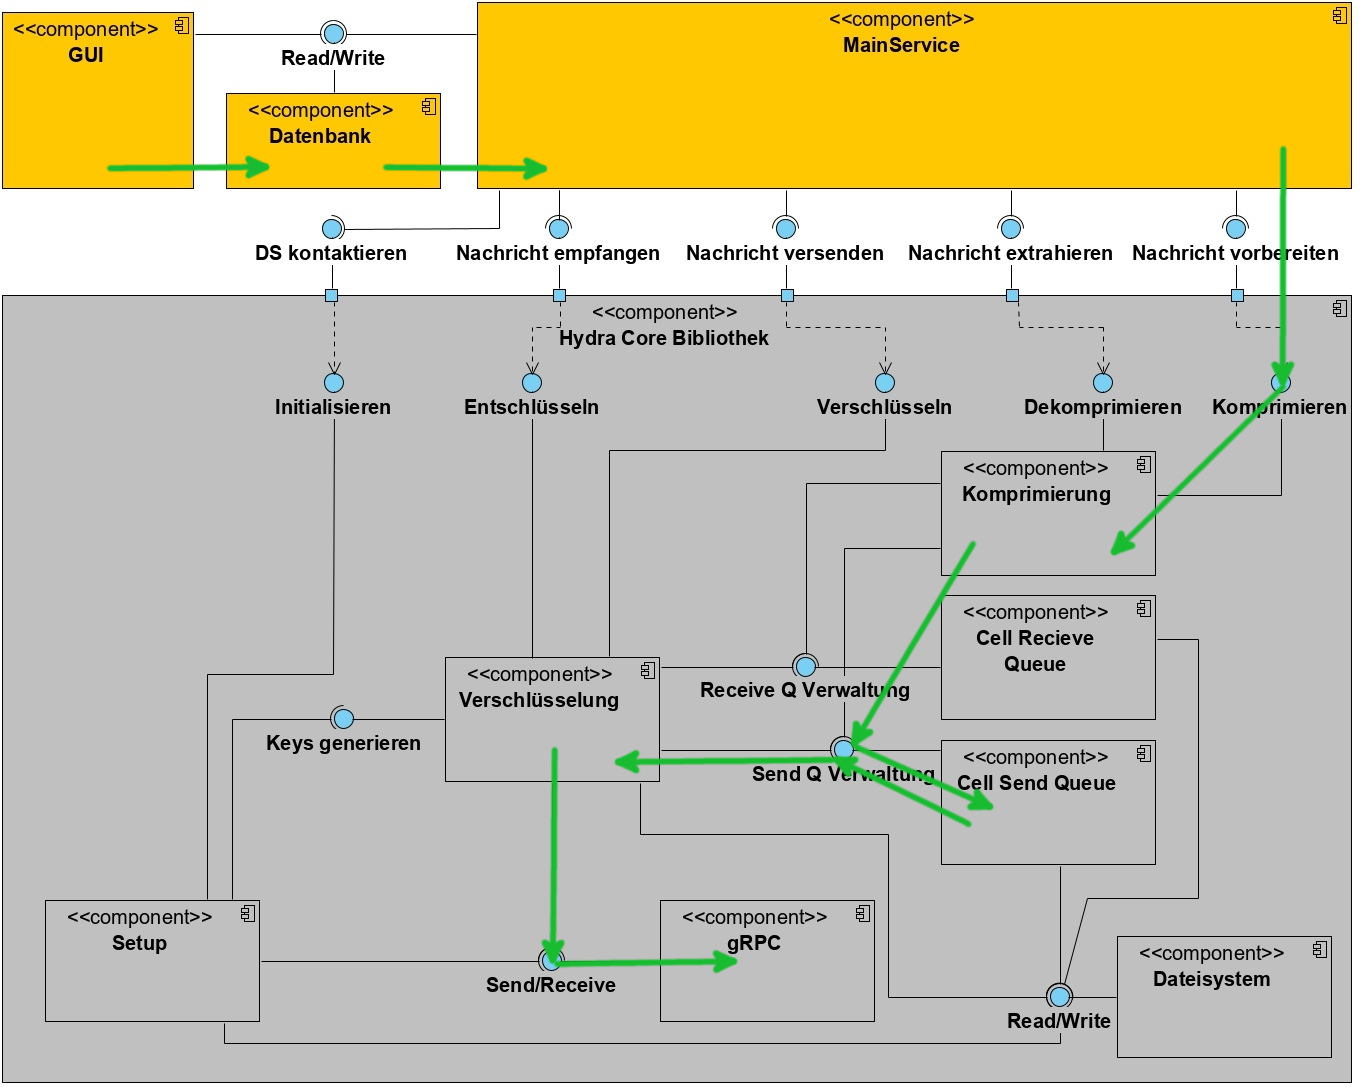
\includegraphics[width=0.9\textwidth]{diagramme/Glob_Kontrollfluss_1.jpg}
  \caption{Kontrollfluss Textnachricht versenden}
  \label{fig:Bild5}
\end{figure}

\begin{enumerate}
    \item
        Der Benutzer gibt eine Nachricht in die \ac{GUI} ein.

    \item
        Die Nachricht wird in der verschlüsselten Datenbank abgespeichert.

    \item
        Der \ac{MS} erkennt eine neue Nachricht in der Datenbank und übergibt sie der \ac{HCB}.

    \item
        Die Nachricht wird von UTF-16 zu ASCII komprimiert.

    \item
        Die Nachricht wird in der \ac{CSQ} abgelegt.

    \item
        Die Nachricht wird Fragment für Fragment aus der \ac{CSQ}  genommen. Anschließend wird eine \ac{E2EE} angewandt. Dazu verwenden wir \ac{AES}. Des Weiteren werden die Fragmente in Circuit-Cells gepackt und onion-encrypted.

    \item
        Die Cells werden anschließend mittels \ac{gRPC} versendet.
\end{enumerate}

\newpage
\subsubsection{Nachricht empfangen}

\begin{figure}[h]
  \centering
     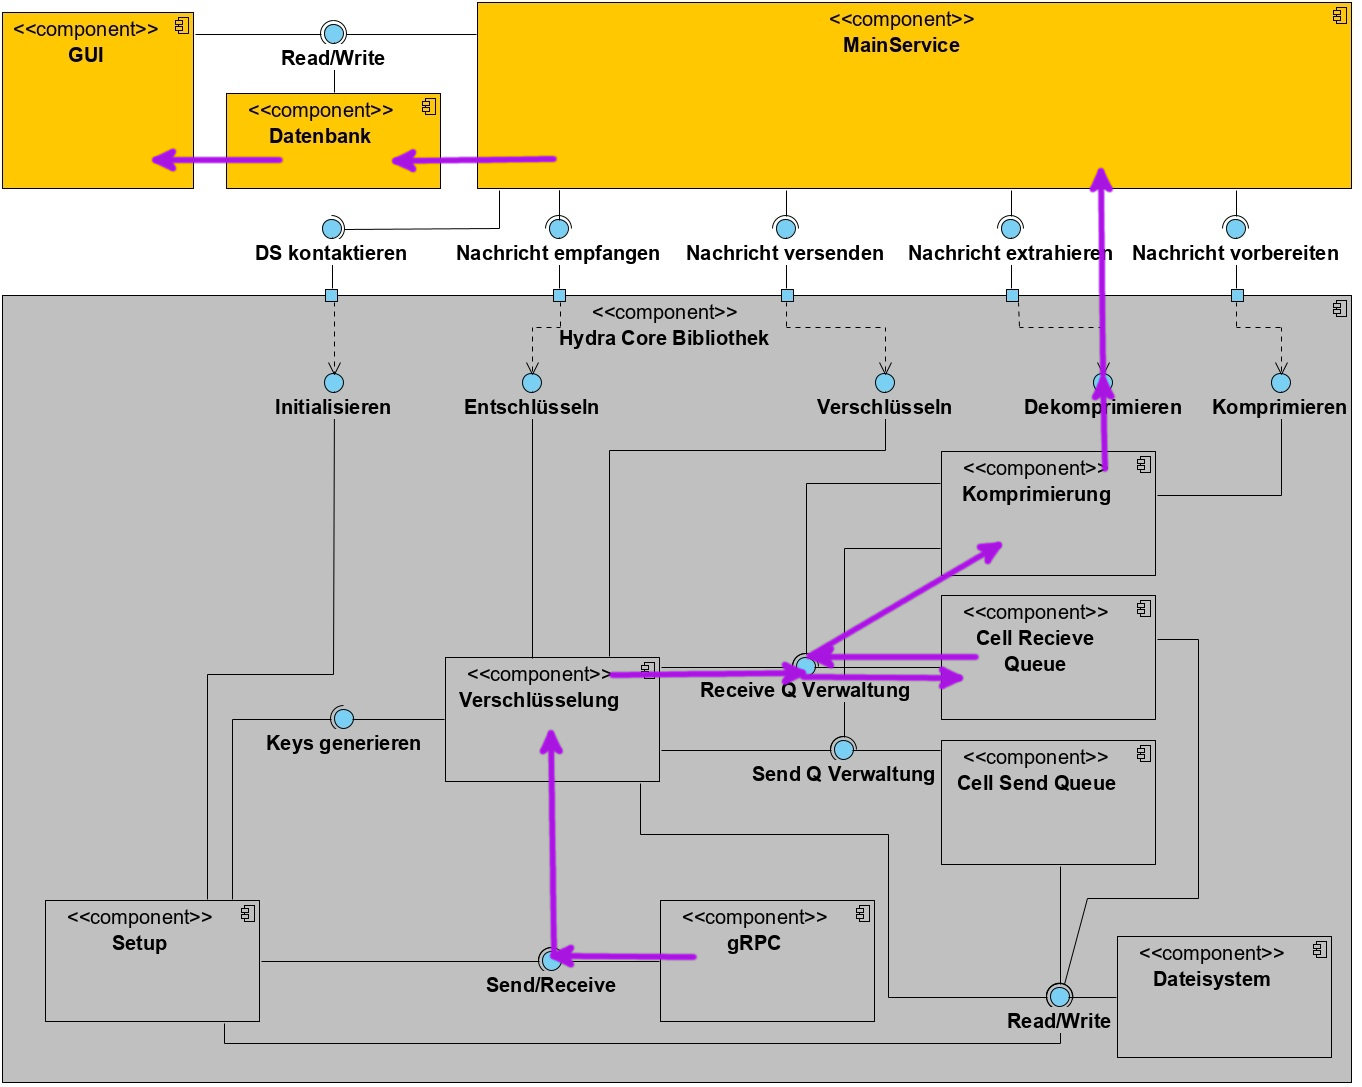
\includegraphics[width=0.9\textwidth]{diagramme/Glob_Kontrollfluss_2.jpg}
  \caption{Kontrollfluss Textnachricht empfangen}
  \label{fig:Bild6}
\end{figure}

\begin{enumerate}
    \item
        Die Cells werden mithilfe von \ac{gRPC} empfangen, dies gewährleistet die \ac{CSQ} des Senders.

    \item
        Die \ac{OE} und \ac{E2EE} werden entfernt.

    \item
        Die Nachricht wird Fragment für Fragment in die \ac{CRQ} geschrieben, bis alle Fragmente angekommen sind. Für jedes, in die \ac{CRQ} eingefügtes Fragment, wird ein Acknowledgement versendet.

    \item
        Die Nachricht wird dekomprimiert.

    \item
        Die Nachricht wird an den \ac{MS} übergeben.

    \item
        Der \ac{MS} speichert die Nachricht in der Datenbank.

    \item
        Die \ac{GUI} liest die Nachricht aus und zeigt sie dem Nutzer an.
\end{enumerate}

\newpage
\subsubsection{\ac{DS} kontaktieren}
 
 \begin{figure}[h]
  \centering
     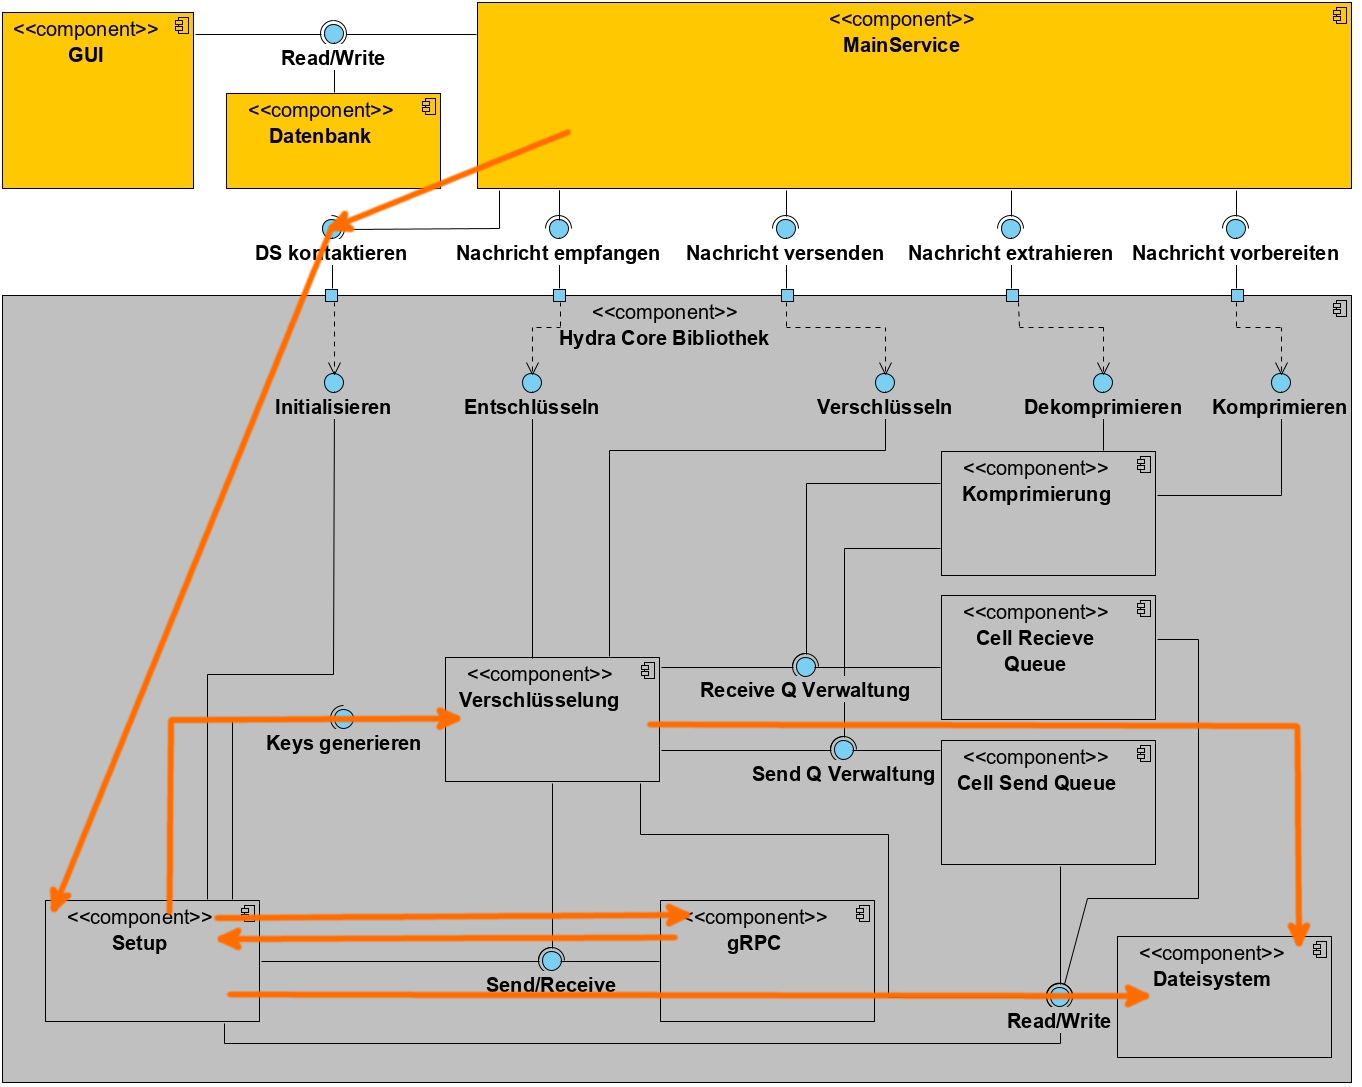
\includegraphics[width=0.9\textwidth]{diagramme/Glob_Kontrollfluss_3.jpg}
  \caption{Kontrollfluss \ac{DS} kontaktieren}
  \label{fig:Bild7}
\end{figure}

\begin{enumerate}
\item Der \ac{MS} ruft die Funktion \textit{\ac{DS} kontaktieren} auf.
\item Das Setup sendet eine Anfrage an der \ac{DS}.
\item Das Setup empfängt die Informationen vom \ac{DS}.
\item Das Setup aktualisiert die Informationen in der Directory-Datei.
\item Das Setup erzeugt für die neuen Epochen jeweils einen neuen Circuit. Dabei wird für jeden neuen Circuit ein Setup-Paket erstellt.
\item Das Setup sendet die erzeugten Setup-Pakets mithilfe von \ac{gRPC} an die dazugehörigen Entry-Mixe.
\item Das Setup lässt sich die neuen onion-Keys für die neuen Epochen von der Komponente \textit{Verschlüsselung} erzeugen und speichert diese in der CircuitKeys-Datei ab.
\end{enumerate}

